\documentclass[12pt,a4paper,danish,oneside,openany]{memoir} 
% Skabelon af DTU's LaTeX support gruppe, v20090423

\usepackage[utf8]{inputenc} 
%\usepackage{usecases}
\usepackage{vhistory}
\usepackage[danish]{babel} % danske overskrifter
\usepackage[T1]{fontenc}   % fonte (output)
\usepackage{lmodern}       % vektor fonte
\usepackage{graphicx}      % indsættelse af billeder
\graphicspath{ {./Figurer/} }
\usepackage{pdfpages}      % pdf som forside evt
\usepackage{morefloats}    % flere floats til tabeller
\usepackage{array}         % udvidet tabel 
\usepackage{listings}      % kode
% \usepackage{palatino}      % lækker font
% \linespread{1.3}           % kræver lidt mere line spacing
\usepackage{rotating}
\usepackage{tikz}

\addto\captionsdanish{
  \renewcommand{\contentsname}%
    {Indholdsfortegnelse}     %
} % Så bruger vi bare 'Indholdsfortegnelse' i stedet for 'Indhold'

\usepackage{underscore}
\usepackage{a4wide}
\usepackage{mathtools} % matematik - underst¿tter muligheden for at bruge \eqref{}

\usepackage[plainpages=false,pdfpagelabels,pageanchor=false]{hyperref} % aktive links

\usepackage{memhfixc}  % rettelser til hyperref

\usepackage{tipa}
\pretolerance=2500     % højt tal, mindre orddeling og mere space mellem ord.
% 3000 er okey, 1000 er for lidt, 5000 i overkanten, 8000 er for meget..

\usepackage[font=small,labelfont=bf,labelsep=endash]{caption}
 
\pagestyle{headings}

\makechapterstyle{mortenovi}{%
\setlength{\beforechapskip}{0cm}%længde fra top af side til kapitel-overskrifter
\setlength{\afterchapskip}{1cm}%længde fra kapiteltekst til body-tekst
\setlength{\midchapskip}{2cm}%længe mellem kapitelnummer og kapiteltekst
\renewcommand\chapnamefont{\normalfont\Large\scshape\raggedleft}
\renewcommand\chaptitlefont{\normalfont\Huge\bfseries\sffamily}
\renewcommand\chapternamenum{}%default "kapitel"
\renewcommand\printchapternum{%
    \makebox[0pt][l]{%
    \hspace{0.4em}
    \resizebox{!}{4ex}{\chapnamefont\bfseries\sffamily\thechapter}}
    }%"kapitel. x"-linjen og dens boxe og bredder - prøv at sætte xyz ind først på de tre linjer respektivt.
\renewcommand\afterchapternum{\par\hspace{1.5cm}\hrule\vspace{0.5cm}}
\renewcommand\afterchaptertitle{\vskip\onelineskip \hrule\vskip\afterchapskip
}}
\chapterstyle{mortenovi}

\maxtocdepth{subsection} %Only parts, chapters and sections in the table of contents
\settocdepth{subsection}

% \includeonly{forord,testing} % Kompiler kun de kapitler du arbejder med.

\topmargin = 0pt
\usepackage[textwidth = 155mm]{geometry}
\usepackage{tabularx}
\usepackage{booktabs} % http://ctan.org/pkg/booktabs 
\newcommand{\tabitem}{~~\llap{\textbullet}~~}

\begin{document}

\part*{Requirements Analysis Document}


%\chapter*{Introduction}

%\section*{Purpose of the system}

%\section*{Scope of the system}

%\section*{Objectives and success criteria of the project}


%\section*{Definitions, acronyms, and abbreviations}

%\section*{References}

%\section*{Overview}


%\chapter*{Current system}


\chapter*{Proposed system}

\section*{Functional requirements}

\subsection*{Calender}
The Calendar is used to keep track of events, e.g. Work calendar or Holiday calendar. The Calendar contains events specific to only itself.
A new calendar is initiated by the Client with a name that described the calendar. The Calendar can be modified by the Client.
 A Calendar may contain one or more events. The system can contain multiple calendars.

\subsection*{Event}
An Event has a start date and an end date.
An Event belongs to a Calendar. Events are initiated by the Client and can also be modified by the Client.
An Event may repeat on multiple dates, e.g. every week/month.
Events have alarms that be set to notify the user

\subsection*{Client}
The Client manages both the Calendars and the Events.
The Client has access to all of his Calendars and Events and can therefore create, edit, share and delete Calendars and Events.
The Client can change the view.
The Client has the ability to Hide/Show different Calendars of their liking.
The Client can synchronize the Calendars with the Server to they are easily accessible on different devices.
The Client has the opportunity to search for specific events.

\subsection*{Server}
The Server is responsible for keeping the Client’s calendars up to date.
When an Event or Calendar is shared the Server must send an invitation to the recipient(s).

\subsection*{Other user}
The Other User receives invitations from the Client and can choose to either accept or decline the invitation.

\subsection*{View}
The are four types of view: Day View, Week View, Month View, Year View.
Besides the view can show one or more Calendars at the same time.

\pagebreak
\section*{Nonfunctional requirements}

\subsection*{Usability}
\begin{itemize}
	\item The user should have basic experience using computers.
	\item The user should be familiar with popular OS interfaces, e.g. Windows 7 or 8.
	\item The user should be able to use the system without little or no documentation.
\end{itemize}


\subsection*{Reliability}
\begin{itemize}
	\item It is important that the Calendars are synchronized.
	\item Restarting of the system is acceptable in the event of a failure.
	\item The system may lost at most five of the last changes made by the user in the event of failure.
\end{itemize}

\subsection*{Performance}
\begin{itemize}
	\item The system should be responsive. There should be little to no latency during actions.
	\item Server synchronization should take no longer than 1-2 minutes on an average home internet connection.
	\item The system should support different user accounts on a computer.
\end{itemize}

\subsection*{Supportability}
\begin{itemize}
	\item Extensions could be the support of other types of Calendar systems, such as GMail, Yahoo Mail etc
\end{itemize}

\subsection*{Implementation}
\begin{itemize}
	\item Internet connection is needed for synchronizing with the server. If no internet connection is available the data is only stored locally.
\end{itemize}

\subsection*{Interface}
\begin{itemize}
	\item The data is saved locally and on the server.
\end{itemize}

\subsection*{Operation}
\begin{itemize}
	\item The user manages the system.
\end{itemize}

\subsection*{Package}
\begin{itemize}
	\item The system is installed by the user.
\end{itemize}

\pagebreak
\section*{System models}

\subsection*{Scenarios}

1: 
Nicolai just got an offer for a new job and wants to delete his old work calendar and replace it with a new one. Nicolai opens his calendar system and selects his old work calendar. He then searches for events he wants to transfer to his new calendar. He finds two events in the old work calendar he wants to transfer to his new calendar. Nicolai then creates a new calendar and creates his first event. While creating his second event, he gets a message saying his job offer is rejected. Luckily Nicolai didn’t quit his old job, so he decides to synchronize his calendar to see if the old one is still on the server.

2:
Peter has a bad day. Just as he is editing his calendar the lightning strikes down in the tree in the backyard and the power goes down and the computer crashes. Peter tries to reboot the computer but the computer will not start. Peter concludes the smoke from the hardware means his computer is now broken. The following week Peter gets himself a new computer. Peter installs the calendar system again and is annoyed that all his calendars are lost. But then Peter remembers that the calendars are stored on the server and that the calendars are not lost.
Peter synchronizes his calendar system with the server and all his calendars are restored.

\pagebreak

\subsection*{Use case model}

\subsubsection{Use case diagrams}

\begin{figure}[ht!]
\centering
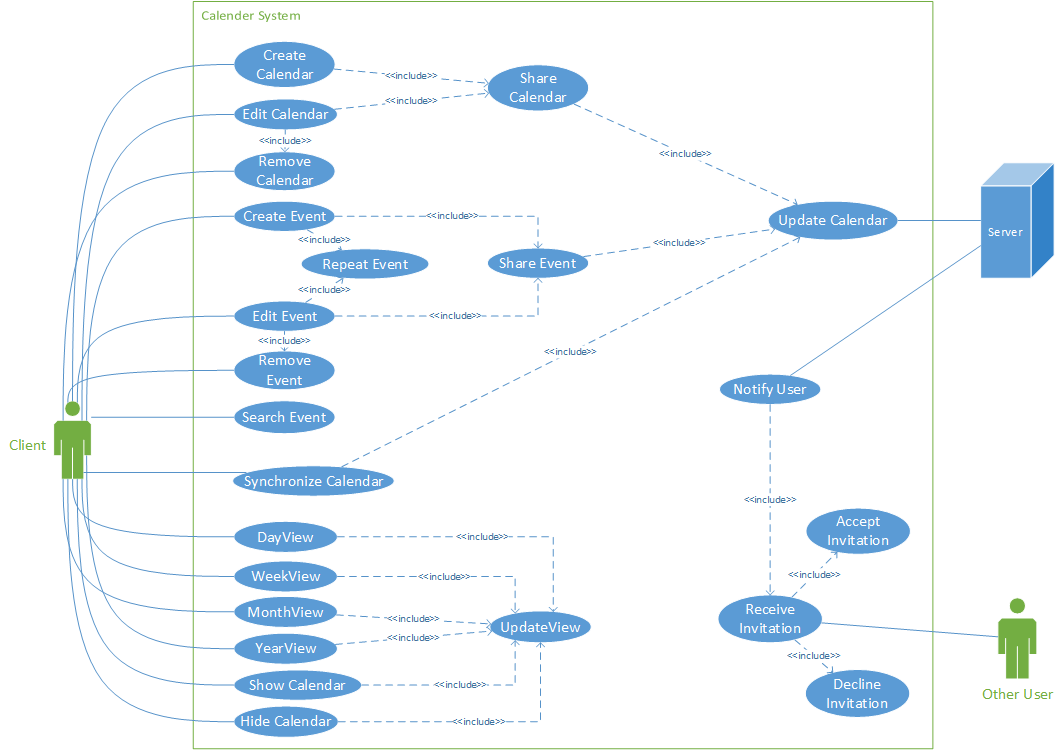
\includegraphics[width=160mm]{usecase.png}
\caption{UML Use Case Diagram \label{overflow}}
\end{figure}

\pagebreak

\subsubsection{Use case tabels}

\begin{usecase}

\addtitle{Use case name}{Create a repeating event } 

\addfield{Participating Actors:}{Initiated by Client \newline Communicates with Server}

\addscenario{Flow of events:}{
	\item The CLIENT creates a new event
	\item The CLIENT Fills out event form
	\item The CLIENT Clicks repeat
	\item The CLIENT Selects interval
	\item The CLIENT Saves Event. \newline - SERVER Synchronizes calendar
}

\additemizedfield{Entry conditions:}{
	\item Calendar must exist in the CLIENT’s user profile
}

\additemizedfield{Exit conditions:}{
	\item Event must have been saved by the CLIENT
	\item Calendar must be synchronized with the SERVER
}

\caption{Use case tabel 1 \label{overflow}}
\end{usecase}

\pagebreak

\begin{usecase}

\addtitle{Use case name}{Share an existing event with another user} 

\addfield{Participating Actors:}{Initiated by Client \newline Communicates with Server and Other_User}

\addscenario{Flow of events:}{
	\item The CLIENT chooses an event.
	\item The CLIENT clicks Edit Event button
	\item The CLIENT clicks on the SHARE button.
	\item The CLIENT enters the username or email of another user he would like to share his event with.
	\item The CLIENT clicks the SEND button.
	\newline - The SERVER sends an invitation to the OTHER_USER.
	\newline - The SERVER sends a notification “Event shared” to the CLIENT.
	\item The CLIENT reads the notification from the SERVER.
	\item The CLIENT closes the notification.
}

\additemizedfield{Entry conditions:}{
	\item The CLIENT must have an existing event.
	\item The CLIENT must be connected to the internet.
	\item The CLIENT must know the email or username of the recipient. 

}

\additemizedfield{Exit conditions:}{
	\item The OTHER_USER must have received the invitation. 
}
\caption{Use case tabel 2 \label{overflow}}
\end{usecase}

\pagebreak

\begin{usecase}

\addtitle{Use case name}{Set two reminders on an existing event} 

\addfield{Participating Actors:}{Initiated by Client \newline Communicates with Server}

\addscenario{Flow of events:}{
	\item The CLIENT chooses an event
	\item The CLIENT clicks Edit Event button
	\item The CLIENT clicks Set Reminder
	\item The CLIENT selects two reminders
	\item The CLIENT sets the time when the reminder should notify the client
	\item The CLIENT chooses Reminder Type ‘Email’ for reminder 1 and   Reminder Type ‘Notification’ for reminder 2
	\item The CLIENT saves the event
	\item The SERVER sends an email to the CLIENT when the first reminder is fired
	\item The SERVER notifies the CLIENT when the second reminder is fired

}

\additemizedfield{Entry conditions:}{
	\item The CLIENT must have a calendar with a future existing event
	\item The CLIENT must have a live connection to the internet

}

\additemizedfield{Exit conditions:}{
	\item The CLIENT must be able to add reminders to an event
}
\caption{Use case tabel 3 \label{overflow}}
\end{usecase}


\newpage
\subsection*{Analysis Object Model}
\subsubsection{Identifying entity, boundary, and control objects}

\begin{tabular}{|l|p{5.3cm}|p{5.3cm}|}
\hline
\multicolumn{3}{|c|}{Identifying Entity Objects} \\
\hline
\textbf{Entity Object} & \textbf{Attributes \& Associations} & \textbf{Definitions} \\
\hline
 Client & 
\begin{itemize}
     \item UserName
\end{itemize} &
The actor of the system. He administrates the Calendars and Events in the system. \\ \hline
Calendar & 
\begin{itemize}
	\item Name
	\item SharedGroup
	\item Color
  \end{itemize} & 
A Calendar is a system used to keep track of events, e.g. Work calendar or Holiday calendar. The Calendar contains events specific to only itself. The system can contain multiple calendars.\\ \hline
Event &
\begin{itemize}
	\item Name
	\item SharedGroup
	\item Color
	\item StartDateTime
	\item EndDateTime
	\item Alarm
	\item Place
	\item Description
\end{itemize} &
An Event is an event belonging to only one Calendar. Events are used to set alarms or reminders. \\ \hline
OtherUser & 
\begin{itemize} 
	\item UserName 
\end{itemize} & 
The actor who receives invitations. He has rights to the other client’s calendar. \\ \hline
Alarm &
\begin{itemize} 
	\item Type
\end{itemize} &
Alarm notify the client within a given amount of time before the event start.  \\ \hline
\end{tabular}

\newpage
\begin{tabular}{|l|p{10cm}|}
\hline
\textbf{Boundary Object} & \textbf{Definition} \\ \hline
CalendarForm & Form used by \textbf{CLIENT} to specify the properties of a \textbf{calendar} during creation or editing. \\ \hline
EventForm & Form used by \textbf{CLIENT} to specify the properties of an \textbf{event} during creation or editing. \\ \hline
ShareForm & Form used by \textbf{CLIENT} to specify the users that the client would like to share his calendar or event with. \\ \hline
InviteNotice & Notice received by \textbf{users} who have been invited to see an \textbf{event} or \textbf{calendar}. \\ \hline
InviteReply & Notice received by \textbf{CLIENT} that informs whether the user has accepted or declined the invite.   \\ \hline
SynchronizedNotice & Notice provided by the \textbf{SERVER} when the \textbf{CLIENT} asked for synchronizing whenever it succeed or fail.  \\ \hline
\end{tabular}


\begin{tabular}{|l|p{10cm}|}
\hline
\textbf{Control Object} & \textbf{Definition} \\ \hline
CalendarControl & 
Manages the reporting function for whenever a \textbf{calendar} is created, edited og removed. 
When a \textbf{calendar} is created, edited or removed the CalendarControl creates a CalendarForm and present it to the \textbf{CLIENT}. It then creates a ShareForm and present it to the \textbf{CLIENT}. It submits the forms and then waits for the \textbf{SERVER} to automatically update( or if the \textbf{CLIENT} synchronizes). The UpdateControl takes over from here. \\ \hline
EventControl & 
Manages the reporting function for whenever an \textbf{event} is created, edited, or removed. 
When an \textbf{event} is created, edited or removed the EventControl creates a EventForm and present it to the \textbf{CLIENT}. It then creates a ShareForm and present it to the \textbf{CLIENT}. It submits the forms and then waits for the \textbf{SERVER} to automatically update( or if the \textbf{CLIENT} synchronizes). The UpdateControl takes over from here. \\ \hline
UpdateControl & 
Manages updates and synchronizations. When a form is submitted the UpdateControl takes over. It waits for the \textbf{SERVER} to automatically update or if the user manually synchronizes. 
When the \textbf{SERVER} updates the \textbf{calendar} the UpdateControl creates a SynchronizedNotice and displays it to the \textbf{CLIENT}. \\ \hline
NotifyUserControl & 
Manages invitation notices and replies. 
If a \textbf{calendar} or \textbf{event} is shared the NotifyUserControl creates an InviteNotice when the system updates. It sends the InviteNotice and creates a InviteReply and waits for the \textbf{OtherUser}’s reply. When the \textbf{OtherUser} give a reply it is displayed to the \textbf{CLIENT}. \\ \hline
\end{tabular}

\newpage
\paragraph{Association Class Diagram}
This diagram is described in the Control Object Table. It illustrates the association between Entity objects, Boundary objects and Control Objects.
\begin{figure}[ht!]
\centering
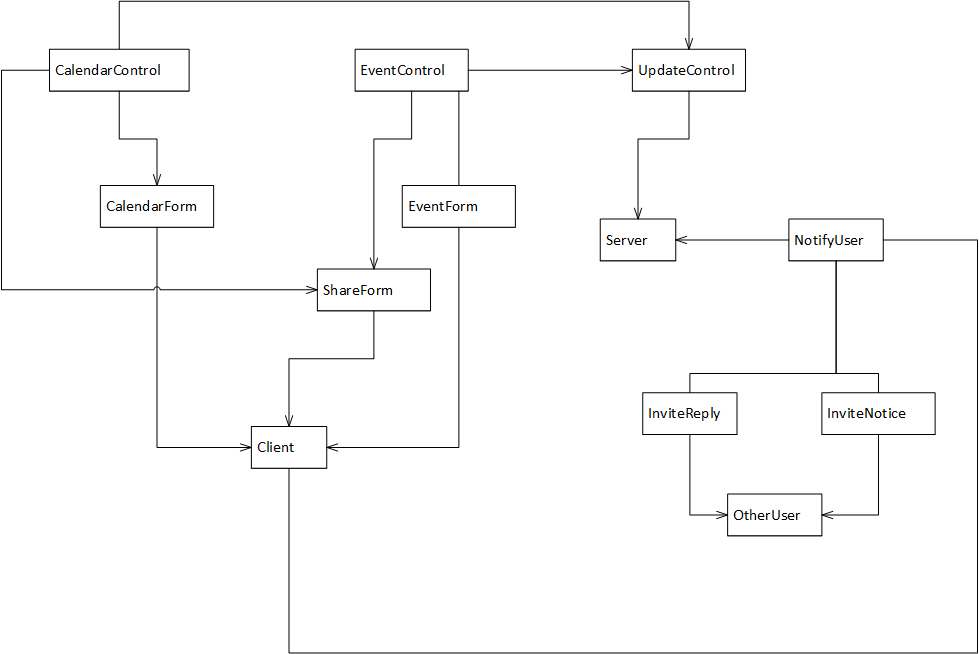
\includegraphics[width=160mm]{diagram.png}
\caption{Association Class Diagram \label{overflow}}
\end{figure}

\newpage
\subsubsection*{Class model}
\begin{figure}[ht!]
\centering
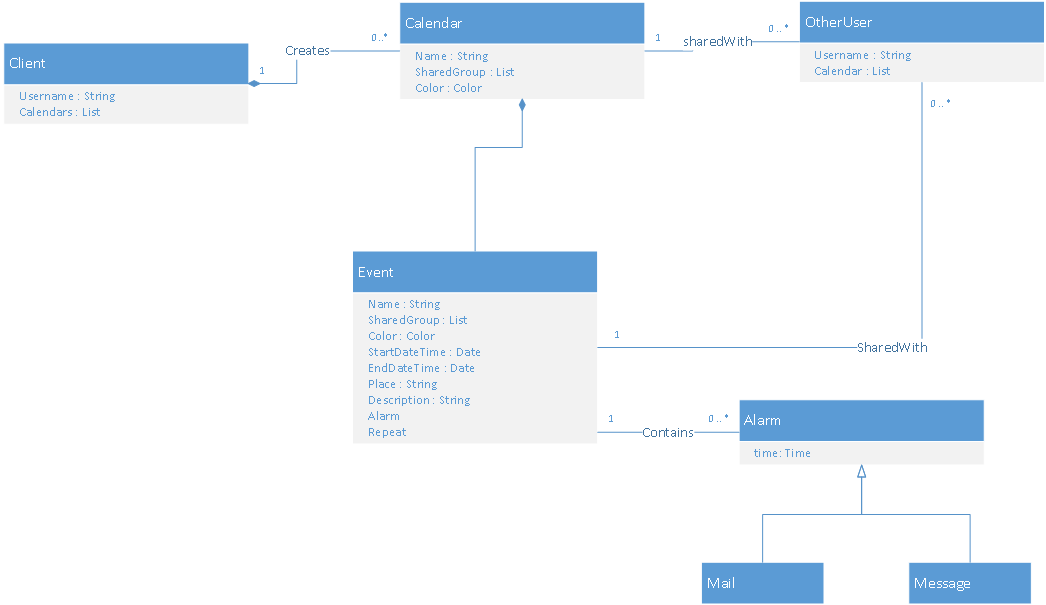
\includegraphics[width=160mm]{class.png}
\caption{UML Class Diagram \label{overflow}}
\end{figure}

\newpage
\subsection*{Dynamic model}
\subsubsection*{Sequence Diagram}

\begin{figure}[ht!]
\centering
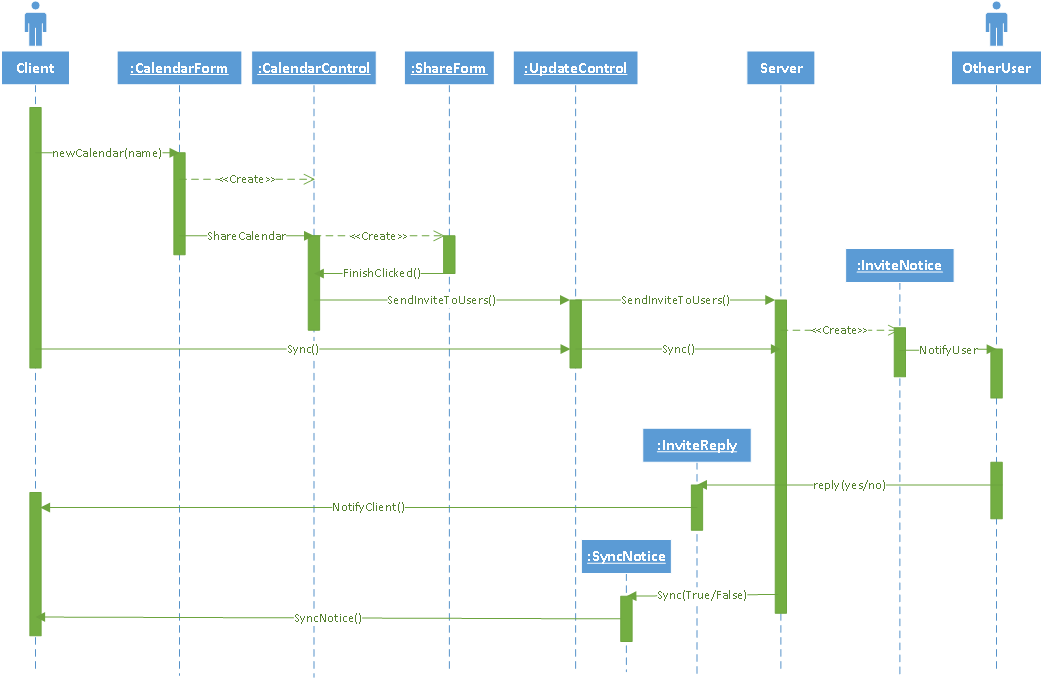
\includegraphics[width=160mm]{scalendar.png}
\caption{Sequence Diagram Calendar Workflow  \label{overflow}}
\end{figure}

\newpage
\begin{figure}[ht!]
\centering
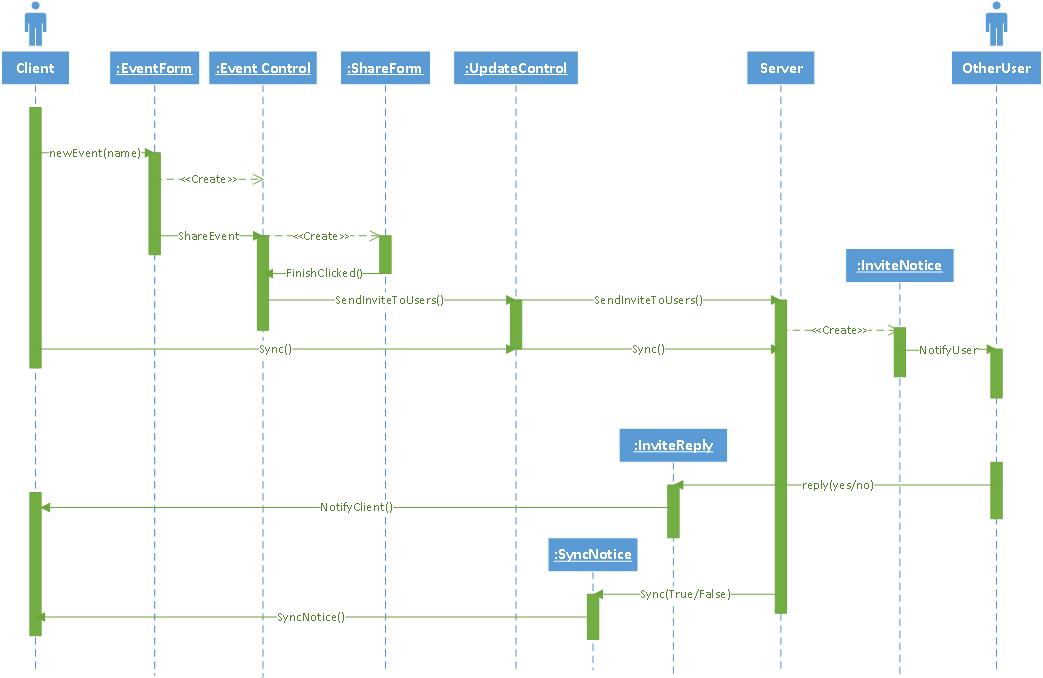
\includegraphics[width=160mm]{sevent.png}
\caption{Sequence Diagram Event Workflow  \label{overflow}}
\end{figure} 


\newpage
\subsubsection*{State Machine Diagram}
\begin{figure}[ht!]
\centering
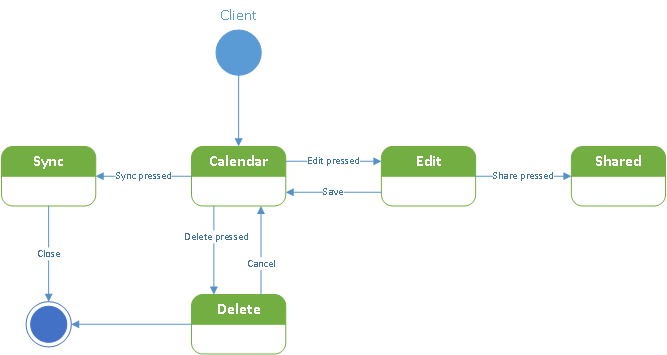
\includegraphics[width=160mm]{calendar.png}
\caption{State Machine Calendar Object  \label{overflow}}
\end{figure}

\begin{figure}[ht!]
\centering
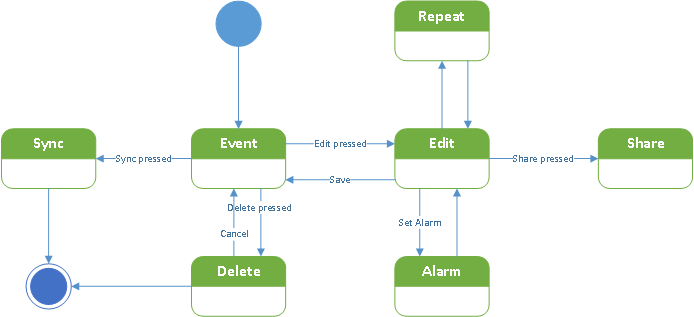
\includegraphics[width=160mm]{event.png}
\caption{State Machine Event Object \label{overflow}}
\end{figure}

\newpage
\begin{figure}[ht!]
\centering
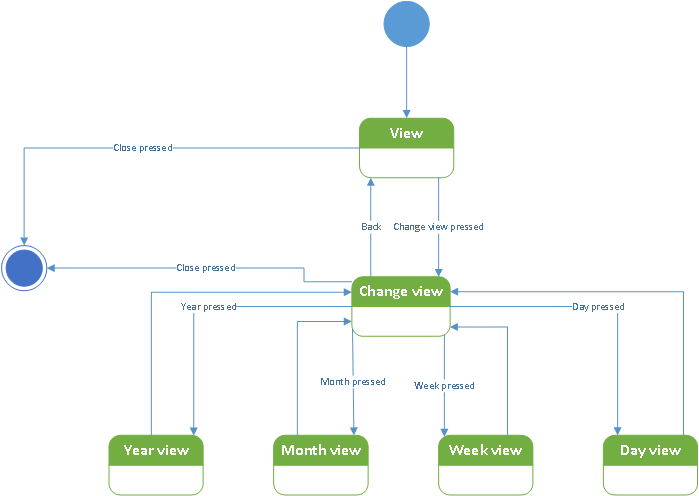
\includegraphics[width=160mm]{view.png}
\caption{State Machine View Object  \label{overflow}}
\end{figure}

%\subsection*{User interface - navigational paths and screen mock-ups}

%\chapter*{Glossary}

\end{document}